\documentclass[10pt,twocolumn,letterpaper]{article}

\usepackage{cvpr}
\usepackage{times}
\usepackage{epsfig}
\usepackage{graphicx}
\usepackage{amsmath}
\usepackage{amssymb}

% Include other packages here, before hyperref.

% If you comment hyperref and then uncomment it, you should delete
% egpaper.aux before re-running latex.  (Or just hit 'q' on the first latex
% run, let it finish, and you should be clear).
\usepackage[breaklinks=true,bookmarks=false]{hyperref}

\cvprfinalcopy % *** Uncomment this line for the final submission

\def\cvprPaperID{****} % *** Enter the CVPR Paper ID here
\def\httilde{\mbox{\tt\raisebox{-.5ex}{\symbol{126}}}}

% Pages are numbered in submission mode, and unnumbered in camera-ready
%\ifcvprfinal\pagestyle{empty}\fi
\setcounter{page}{4321}
\begin{document}

%%%%%%%%% TITLE
\title{Video Compression with 3D Convolutional Neural Networks}

\author{Brennan Shacklett\\
Stanford University\\
Stanford, CA\\
{\tt\small bps@cs.stanford.edu}
% For a paper whose authors are all at the same institution,
% omit the following lines up until the closing ``}''.
% Additional authors and addresses can be added with ``\and'',
% just like the second author.
% To save space, use either the email address or home page, not both
}

\maketitle
%\thispagestyle{empty}

%%%%%%%%% ABSTRACT
\begin{abstract}
  Video compression is an increasingly important area of research due to demands from online streaming applications. Conventional lossy compression algorithms exploit both spatial and temporal redundancy within videos to achieve large compression savings; however, these algorithms are the product of extensive fine tuning and careful approximations, which can make further innovation difficult. Rather than a conventional video compression scheme, this work uses a 3D Convolutional Neural Network combined with an autoencoded residual to learn the relationship between sections of video and generate a prediction of the next frame. Only the autoencoder's internal representation is necessary to decode videos in this scheme, which enables considerable compression savings with relatively little distortion on many scenes as measured by MS-SSIM, particularly in low bitrate contexts.
\end{abstract}

%%%%%%%%% BODY TEXT
\section{Introduction}

As the resolution and framerate demands of both viewers and content creators increase, the bandwidth and computation demands of online video streaming continue to grow. While transferring raw video data is impractical due to massive bandwidth requirements, in a typical video the current frame is closely correlated with the previous frame in a video, since typically the camera and scene will only have moved slightly in the interval between frames. Modern lossy video compression algorithms are able to exploit this temporal redundancy to achieve considerable compression savings with minimal distortion.

Current video codecs are the product of many years of fine tuning and careful approximations, which can make development of innovative new techniques difficult without breaking the finely tuned balance of a wide variety of different codec features. Additionally, in modern codecs, compression savings have come out the cost of ever increasing computational demands: AV1, a state of the art codec achieves around 50\% compression savings when compared to VP9 (a previous gen codec), but this comes at the cost of 4-10 times the encoding complexity [https://streaminglearningcenter.com/codecs/netflix-on-av1.html].

One important note is that despite this increasing computational complexity, these codecs do not attempt to make ``intelligent'' predictions of the next frame based on the current frame's visual information. Instead, codecs contain a large library of different prediction modes, which each perform a relatively simple prediction such as copying pixels from one block of video to another. The optimal mode is then selected by the encoder and transmitted to the decoder as part of the compressed video: therefore most of the complexity in modern video encoders --- both from a design and a computation standpoint --- comes from intelligently selecting the optimal mode for each section of video.

Given the success of neural networks in interpreting visual data, and generating new visual data, it seems natural that neural networks should be able to improve upon the techniques used in conventional video codecs. Furthermore, the automatic nature of neural network optimization means that neural network based video encoders should considerably reduce the difficulty of experimenting and innovating in this field, since new network structures can be quickly optimized and tested when compared to the painstaking process of developing a new feature in a conventional codec.

This work explores one of many possible directions for neural network based video compression: using convolutional neural networks to predict the next frame in a video sequence based on previous frames, combined with CNN based compression of the residual between the predicted frame and the true frame. In this scheme, a given frame in a video sequence is reconstructed by first using a CNN to predict the current frame based on a set number of previous frames, and then decoding the compressed residual and adding it to the prediction. Therefore the complete network takes in the previous $N$ frames along with the current frame as input, and produces a single image --- the reconstruction --- along with the compressed residual.

\section{Related Work}
Although there is extensive literature in the field of conventional video compression, little of it is particularly useful to this work, which aims to build a purely neural network based compression approach. While combining conventional techniques with small neural network based components can be successful as shown by Chen et al \cite{av1improv1} and Fu et al \cite{av1improv2} in their work on adding prediction modes to AV1, such approaches still suffer from the difficulties of choosing features and prediction modes found in conventional codec development. The original paper describing the MPEG codec \cite{LeGall}, provides a good reference for the basic techniques still employed by most conventional video codecs, which can be seen as a baseline for the types of features a neural network based approach needs to emulate in order to be successful. For the purposes of this project, the key emulated features are prediction from previous frames and compression of the residual. One key component of traditional compression is probalistic entropy coding as the final step of compression in order to ensure as dense a binary representation as possible; however for simplicity this was not explored in the project.

In recent years, there has been growing interest in applying neural networks to compression problems, but thus far most work has focused on single image compression rather than video. Two relatively recent papers from Wu et al \cite{DBLP:journals/corr/abs-1804-06919} and Chen et al \cite{DBLP:journals/corr/abs-1804-09869} describe deep learning based video compression schemes, but both require external motion estimation algorithms rather than learning motion prediction in the network. Since motion prediction --- the process of predicting where pixels from previous frames should be placed in the next frame --- is the key source of removing temporal redundancy in video compression, this project aimed to avoid offloading this step to a external algorithm. Instead, inspired by the success of 3D CNNs for video action recognition and segmentation in \cite{DBLP:journals/corr/abs-1712-01111}, as well as the use of 3D CNNs for image sequence block matching and denoising in \cite{DBLP:journals/corr/AhnC17}, this project relies on 3D CNNs to perform motion prediction.

Both Wu et al and Chen et al also rely on dividing the video into a series of fixed size blocks rather than operating on entire frames, which allows deeper networks to be possible without unrealistic computation demands. This approach is also used extensively in conventional video compression, where each frame is divided into spatially correlated blocks and subblocks to allow many different prediction modes in the same frame. Due to the success of dividing into blocks in these papers as well as in conventional compression, this project also divides the input video into fixed size blocks, which reduces the memory footprint of the networks and effectively increases the amount of training data available.

After the prediction step, these learning based video compression schemes rely on techniques similar to ones used in single image compression in order to compress the remaining information required for reconstruction of a video frame. Work by Toderici et al \cite{DBLP:journals/corr/TodericiVJHMSC16}\cite{DBLP:journals/corr/TodericiOHVMBCS15} on neural network based image compression shows the success of various autoencoder and LSTM based approaches for compressing images in 32 by 32 pixel blocks with variable compression rates. These schemes are able to support variable compression rates by additively encoding the image. Rather than simply allowing one pass through the network for each pixel block, the residual for a given block can be passed back through the network to reduce errors at the cost of less compression. Although Toderici et al's work concludes that using convolutional LSTMs is currently the optimal approach for image compression, this project uses a network based on their convolutional autoencoder structure for compressing the residual, due to its relative simplicity and easier training. Newer work by Minnen et al \cite{Minnen} demonstrates how to extend these schemes to allow variable entropy encoding for each block of an image; however while this would undoubtedly improve the performance of this project, it has to be left as a future extension.

\section{Dataset \& Features}
The core dataset used for this project is the \texttt{objective-2-slow} dataset from the Xiph Foundation \cite{xiph}. This dataset contains 75 raw uncompressed videos ranging in resolution from 360p to 4K, and spanning between 30 and 120 frames. A partner dataset from the Xiph Foundation named \texttt{objective-2-fast} also exists, which contains a subset of the videos from \texttt{objective-2-slow} and is designed for faster testing purposes. For the purposes of this project, the \texttt{objective-2-fast} dataset was divided into four parts, with the first part being the test set and the second part being the validation set, and the 3rd and 4th parts combined into the training set along with all the videos from \texttt{objective-2-slow} (except the videos from objective-2-slow already used in testing or validation). Additionally, the testing dataset was combined with long sequences from the Blender Foundation's Big Buck Bunny and Sintel animated movies \cite{blender}, in order to test the algorithms on much longer videos. The testing and validation sets were then divided into a larger number of short sequences to ensure that each had a relatively wide variety of different clips.

This left approximately 50 videos in the training set, fifteen 30 frame videos in the validation set, and fifteen 30 frame videos in the test set (plus the 2 long sequences in the test set). Although these numbers are quite low, all the tested networks operate on each 32x32 block of pixels in the video independently. Since most of the videos are 4K or 1080p, this means the dataset had a very large number of separate 32x32 blocks (approximately 9000 individual blocks for a single frame of a 4K video) to train and test on. Unfortunately many of these blocks are quite similar, especially in high resolution videos where each block represents a relatively small portion of the scene.

\begin{figure}[t]
\begin{center}
  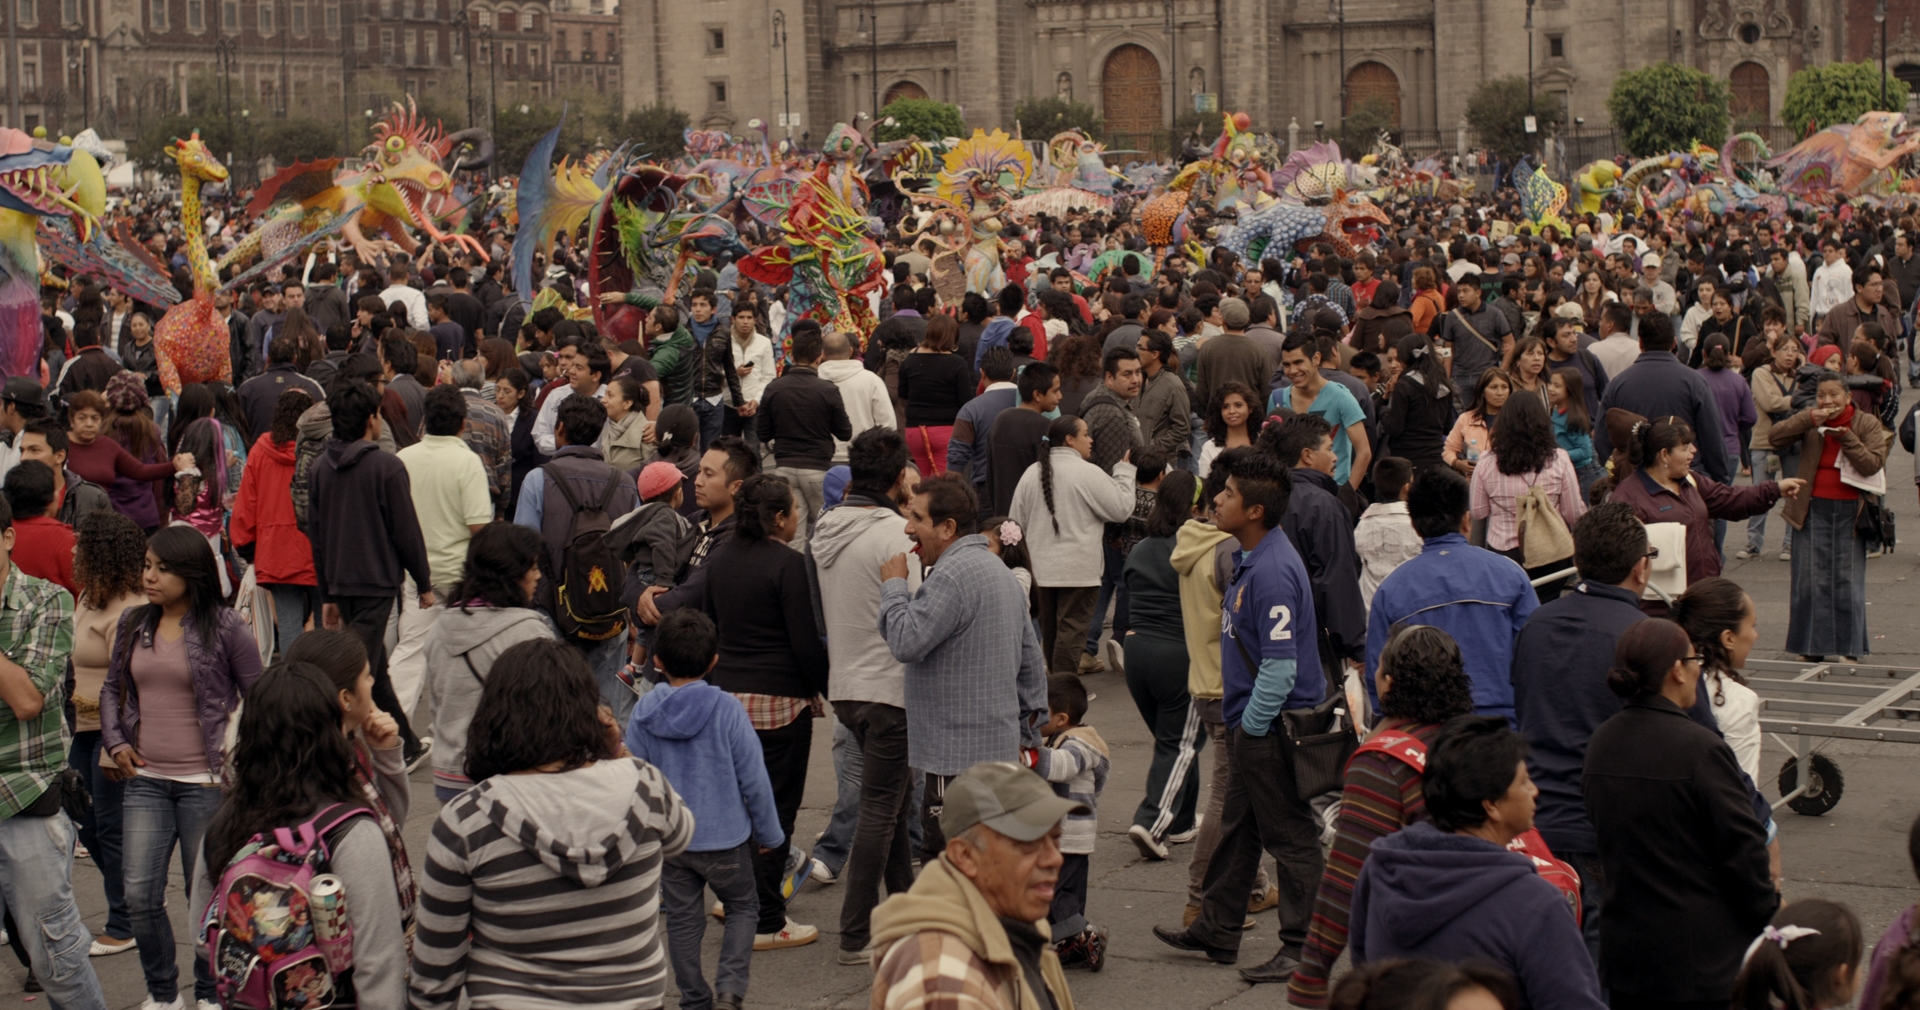
\includegraphics[width=0.8\linewidth]{data_example}
\end{center}
   \caption{Example of a frame in 4K video from the \texttt{objective-2-slow} dataset.}
\end{figure}

In terms of preprocessing, each video was padded to have both the width and height be multiples of 32, so the network did not have to handle any non square sections of video on the edges; however, this padding was removed for the final distortion metrics on the test set. Additionally the per channel means and standard deviation were computed across the training set for normalization purposes. For efficiency purposes during training, the training set was also transformed to allow stacking multiple independent 32x32 pixel blocks from a given frame together into a single training batch, since different video lengths and sizes made processing different videos in the same batch inefficient. All the source videos were originally stored in YUV 4:2:0 color format meaning one channel for brightness information (luma), and then two half width and half height color (chroma) channels. This is known as chroma subsampling \cite{van2001vision} and is standard practice for conventional video compression, since the human eye has a greater sensitivity to brightness than color information. Unfortunately video data where different channels have different dimensions does not mesh well with current neural networks, so each frame of video was converted to standard 3 channel RGB, which was used as the only feature for the dataset.

\section{Methods}
This project explored several different network architectures to find a network that could successfully compress and reconstruct video frames with minimal distortion. Despite many variations, the core architecture remained approximately the same, and can be see in Figure \ref{fig:core}. For each 32x32 block in the current frame the following algorithm is run: first, the previous $N$ frames, and possibly part of the current frame are passed into the predictor network, then a residual is computed between the output of the predictor network and the true value of the current 32x32 block. This residual is then passed into an autoencoder that compresses the 32x32 block of residual pixels into a smaller representation, which can then be used by the decoder section of the autoencoder to reconstruct the residual. This reconstructed residual is then added to the the predicted block to create the lossy version of the input block. A slight variation on this approach is to pass the full uncompressed 32x32 pixel block into the autoencoder rather than the residual, and then to sum the prediction with the output of the autoencoder. While this approach would enable more parallelism since the autoencoder and the predictor can work in parallel, initial testing indicated it was inferior to the approach in \ref{fig:core}, so it was abandoned early on.

One of the key features of modern video codecs is their ability to predict a given block of video based on either blocks from previous frames, or already reconstructed blocks within the current frame. 

\section{Experiments \& Results}

{\small
\bibliographystyle{ieee}
\bibliography{egbib}
}

\end{document}
